\section{EXPERIMENTAL DETAILS}
\label{app:experimental}

\subsection{Sections}
\label{app:sections}

\Cref{tab:sections} lists the sections of \cref{sec:setup}, and \cref{fig:sections} shows them. The lineage classes include Unassigned. On the ovarian FFPE section it also holds a low-depth class of mixed lineage that the curated annotation had named as a tumour subtype, which is why its share is the largest.

\begin{table}[t]
\centering
\caption{The sections. Median counts are per cell over the whole section. The TMA core and its serial section are one core of the microarray on two slides; no model is fitted to the serial section.}
\label{tab:sections}
\small
\setlength{\tabcolsep}{4pt}
\begin{tabular}{@{}llrrrrr@{}}
\toprule
Section & Role & Cells & Genes & Lineage classes & Unassigned (\%) & Median counts \\
\midrule
Ovarian cancer (FFPE) & primary & 407{,}120 & 5{,}101 & 12 & 10.3 & 178 \\
Lung cancer (FFPE) & fitted & 278{,}324 & 5{,}001 & 20 & 0.1 & 242 \\
Ovarian cancer (FF) & fitted & 1{,}157{,}637 & 5{,}001 & 10 & 4.3 & 1{,}401 \\
Lung TMA core & fitted & 69{,}422 & 5{,}001 & 30 & 4.2 & 279 \\
Lung TMA core, serial section & held out & 70{,}757 & 5{,}001 & 30 & 4.8 & 253 \\
\bottomrule
\end{tabular}
\end{table}

\begin{figure}[t]
\centering
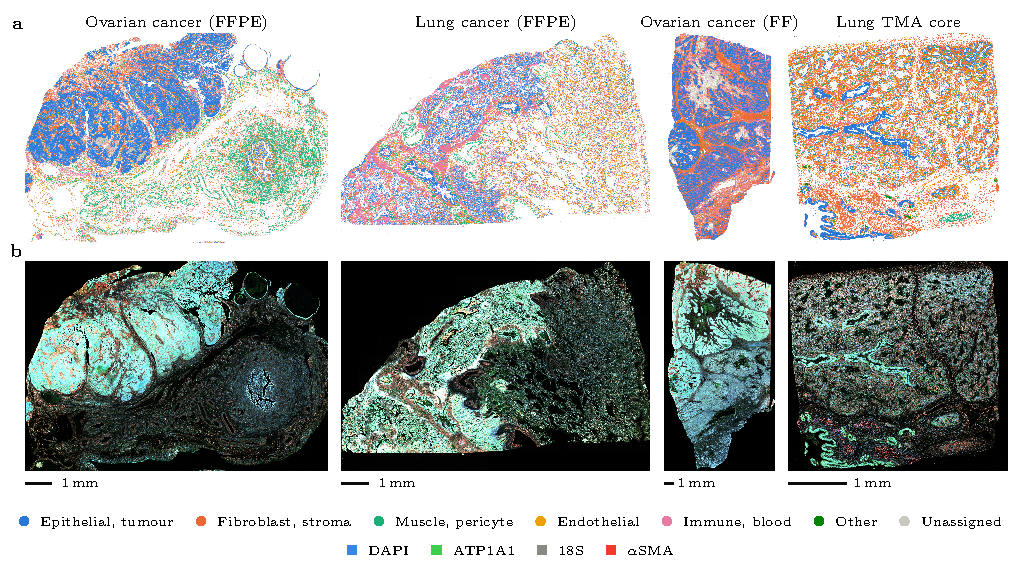
\includegraphics[width=\textwidth]{figures/fig_sections}
\caption{The four fitted sections. \textbf{a},~Every cell at its centroid, coloured by its lineage label, with the labels grouped into six families for display only; the model is fitted with the finer lineage classes of \cref{tab:sections}. \textbf{b},~The morphology image of the same section, the four channels the image descriptor reads, coloured as in \cref{fig:overview}b. The TMA panel is the fitted core only. Each section is shown at its own scale; the bars are $1$\,mm.}
\label{fig:sections}
\end{figure}

\subsection{Lineage Labels}
\label{app:lineage}

The fitted labels are lineage-level on every section (\cref{sec:setting}). States, such as proliferating, activated or hypoxic, and locations, such as tumour- or stroma-associated, are merged into their lineage; lineages and developmentally distinct sub-lineages are kept. The mappings were fixed and recorded before any model was refitted.

\paragraph{Curated annotations.}
On the ovarian FFPE section the eighteen curated classes become twelve (\cref{tab:lineage-ovarian}). Two classes needed a decision. The class named as a SOX2-OT$^+$ tumour subtype is mostly not tumour: its cells have a median of $27$ transcripts against $333$ for tumour cells, three quarters show no SOX2-OT count, and its pooled profile decomposes mostly into macrophage expression, so it is folded into Unassigned rather than into the tumour lineage. The class named as malignant cells lining a cyst expresses mesothelial markers (CALB2, PRG4, BNC1, PDPN, UPK3B) and lacks the tumour markers (EPCAM, PAX8, ESR1), and becomes its own lineage. On the lung TMA the thirty-five curated classes become thirty: the state classes (activated, inflammatory and myofibroblasts, activated endothelium and proliferating cells) are reassigned cell by cell to the sub-lineage their markers indicate, with the cell-cycle genes left out for the proliferating class, and the other classes are kept.

\paragraph{Other judgement calls.}
Four further choices are not forced by the rule and are stated so that they can be revisited. The tumour- and stroma-associated fibroblasts of the ovarian FFPE section are merged, because what separates them is the cancer-associated fibroblast programme, a state, rather than a lineage. Its two endothelial classes are merged too, although what separates them is less clear: a tip-cell state on one side and a weakly venous identity on the other. On the lung TMA the alveolar and adventitial fibroblasts are kept as distinct sub-lineages, and the myofibroblasts, which could belong to either, are split between them by their markers, about evenly. The cell-by-cell reassignment of the TMA's state classes is expected to be right for about three cells in four, and its margins are recorded with the mapping.

\paragraph{Clustered sections.}
On the lung FFPE section and the fresh-frozen ovarian section the labels start from unsupervised clusters, and each cluster is assigned the lineage its marker genes indicate, on the lung TMA's vocabulary for the lung section (\cref{tab:lineage-clusters}). Clusters of immune cells next to tumour that carry some tumour signal keep their immune lineage, since that signal is the leakage the model is built to absorb, and one low-depth cluster of the fresh-frozen section becomes Unassigned.

\begin{table}[t]
\centering
\caption{Lineage labels on the ovarian FFPE section: the curated classes merged into each lineage.}
\label{tab:lineage-ovarian}
\small
\begin{tabular}{@{}>{\raggedright\arraybackslash}p{0.28\textwidth}>{\raggedright\arraybackslash}p{0.62\textwidth}@{}}
\toprule
Lineage & Curated classes \\
\midrule
Ciliated epithelial cells & Ciliated Epithelial Cells \\
Endothelial cells & Stromal Associated Endothelial Cells, Tumor Associated Endothelial Cells \\
Fallopian tube epithelium & Fallopian Tube Epithelium \\
Fibroblasts & Stromal Associated Fibroblasts, Tumor Associated Fibroblasts \\
Macrophages & Macrophages \\
Mesothelial-like cyst lining & Malignant Cells Lining Cyst \\
Pericytes & Pericytes \\
Smooth muscle cells & Smooth Muscle Cells \\
T/NK cells & T and NK Cells \\
Tumour & Inflammatory Tumor Cells, Proliferative Tumor Cells, Tumor Cells, VEGFA+ Tumor Cells \\
Unassigned & SOX2-OT+ Tumor Cells, Unassigned \\
Urothelial-like cells & Urothelial-like Cells \\
\bottomrule
\end{tabular}
\end{table}

\begin{table}[t]
\centering
\caption{Lineage labels on the two clustered sections: the clusters assigned to each lineage.}
\label{tab:lineage-clusters}
\small
\begin{tabular}{@{}>{\raggedright\arraybackslash}p{0.24\textwidth}>{\raggedright\arraybackslash}p{0.13\textwidth}@{\hspace{0.04\textwidth}}>{\raggedright\arraybackslash}p{0.2\textwidth}>{\raggedright\arraybackslash}p{0.33\textwidth}@{}}
\toprule
\multicolumn{2}{@{}l}{Lung cancer (FFPE)} & \multicolumn{2}{l@{}}{Ovarian cancer (FF)} \\
\cmidrule(r){1-2}\cmidrule(l){3-4}
Lineage & Clusters & Lineage & Clusters \\
\midrule
AT1 & 18, 23 & Endothelial cells & 16, 38 \\
AT2 & 20 & Fibroblasts & 7, 13 \\
Adventitial fibroblasts & 4, 17 & Macrophages & 10, 14, 19, 20, 25, 26, 28, 30, 34 \\
Alveolar fibroblasts & 10 & Ovarian stroma & 3, 6, 23 \\
Alveolar macrophages & 16 & Pericytes & 32 \\
B cells & 12 & Plasma cells & 17, 35 \\
EC general capillary & 3, 22, 25 & Smooth muscle cells & 33 \\
EC venous & 13 & T/NK cells & 18, 22, 24, 27, 29, 31, 36, 37 \\
Goblet & 19 & Tumour & 1, 2, 4, 5, 8, 11, 12, 15, 21 \\
Interstitial macrophages & 2 & Unassigned & 9; unclustered cells \\
Mast cells & 27 &  &  \\
Multiciliated & 26, 28 &  &  \\
Neuroendocrine & 31 &  &  \\
Neutrophils & 6 &  &  \\
Pericytes & 24 &  &  \\
Plasma cells & 15 &  &  \\
Smooth muscle & 5 &  &  \\
T/NK cells & 1, 7, 21, 30, 32 &  &  \\
Tumour & 8, 9, 11, 14, 29 &  &  \\
Unassigned & unclustered cells &  &  \\
\bottomrule
\end{tabular}
\end{table}

\subsection{Baselines}
\label{app:baselines}

\Cref{tab:baselines} gives the configuration of each comparison method. Every method is run at its published defaults, and on our pruned Delaunay graph where it accepts an external graph; resolVI and MintFlow build their own. The methods that read a label read the lineage labels. SIMVI does not read one, so refitting it at lineage labels only checks reproducibility.

\begin{table}[t]
\centering
\caption{Comparison methods as run. Versions are the package versions used.}
\label{tab:baselines}
\small
\setlength{\tabcolsep}{4pt}
\begin{tabular}{@{}>{\raggedright\arraybackslash}p{0.11\textwidth}>{\raggedright\arraybackslash}p{0.2\textwidth}>{\raggedright\arraybackslash}p{0.22\textwidth}>{\raggedright\arraybackslash}p{0.13\textwidth}>{\raggedright\arraybackslash}p{0.24\textwidth}@{}}
\toprule
Method & Version & Graph & Label & Budget and coverage \\
\midrule
resolVI & scvi-tools 1.5.1 & own, 10 nearest neighbours & lineage & 50 epochs; every section \\
SIMVI & simvi 0.1.2 (scvi-tools 0.16.1) & ours & not used & package default; the TMA core and its serial section; failed on the fresh-frozen section (the whole section does not fit in GPU memory); not attempted on the two FFPE sections \\
MintFlow & mintflow 0.3.0 & own Delaunay graph & lineage & width 600, 50 epochs; the TMA core, transferred to its serial section; failed on the fresh-frozen section (out of host memory before training); not attempted on the two FFPE sections \\
Cellina & cellina 1.1.1 (scvi-tools 1.2.0) & ours & lineage & package default; being run \\
\bottomrule
\end{tabular}
\end{table}

\subsection{Assets and Licences}
\label{app:assets}

The ovarian FFPE, lung FFPE and fresh-frozen ovarian sections are public datasets of 10x Genomics \citep{tenx_ovarian_ffpe,tenx_lung_ffpe,tenx_ovary_ff}, released under the Creative Commons Attribution 4.0 International licence (CC BY 4.0). The TMA core and its serial section are two samples of GEO series GSE315411 \citep{williamskatek2026fishing}; NCBI places no restriction on the use or distribution of GEO data, while noting that submitters may claim rights in the data they submit \todo{verify the wording on the GEO disclaimer page}. The image model KRONOS and its successor KRONOS2 \citep{kronos2025} are released under CC BY-NC-ND~4.0, for non-commercial academic research and after registration; we use them for that purpose and redistribute neither. The comparison methods are released under the BSD 3-Clause licence: scvi-tools, which contains resolVI, SIMVI, MintFlow and Cellina. The code will be released on acceptance; no new data are released.

\subsection{Training Cost}
\label{app:timing}

\Cref{tab:timing} gives the cost of a fit. DISCELL's time per epoch is pure training, measured over twenty epochs with no evaluation. Its wall-clock time covers the three final fits, including evaluations every five epochs and the early stop. The comparison methods' times are whole fits, as recorded when they were run.

In symbols, a training step on a tile of $n$ seeds with $n_1$ cells in ring one costs $O((n + n_1)\,G h)$ in the encoders and decoder, for hidden width $h$, and $O(|E_n|\,G)$ in the foreign influx, for the $|E_n|$ edges into the seeds (\cref{sec:batching}). The six adversary head updates add $O\big(6\,(n + n_1)\,h_a(\dz + K)\big)$ with $h_a = 64$, small beside the gene-sized terms because $\dz$ and $K$ are far below $G$. An epoch visits every training tile once, so its cost is linear in the number of cells; the held-out probes are fitted on at most $30{,}000$ cells whatever the section's size. Peak memory is the section's count matrix, held resident, plus the gathered edge-by-gene rows of the influx, $O(|E_n|\,G)$ per step, which the tile size bounds. The leakage sweep multiplies the cost of a fit by its six grid points and three seeds, eighteen fits per section. Sample size is not analysed: how many cells a section needs for the readouts to stabilise is not studied beyond the range of sizes in \cref{tab:sections}.

\begin{table}[t]
\centering
\caption{Model size and training cost on one GPU. \emph{Peak memory}: largest allocation during training, with the section resident on the GPU. \emph{Run time}: one whole fit, for DISCELL including its evaluations every five epochs and the early stop, as the range over the three seeds of the final configuration. Where a method has no time, the reason is given: \emph{not attempted} means it was never run on that section, \emph{failed} that it was run and did not complete.}
\label{tab:timing}
\small
\setlength{\tabcolsep}{4pt}
\begin{tabular}{@{}lrrrr@{}}
\toprule
& Ovarian (FFPE) & Lung (FFPE) & Ovarian (FF) & Lung TMA core \\
\midrule
\multicolumn{5}{@{}l}{\emph{DISCELL, model and training details}} \\
\quad parameters (M) & 4.19 & 4.12 & 4.11 & 4.13 \\
\quad peak memory (GiB) & 6.3 & 4.3 & 15.1 & 1.4 \\
\quad epochs to the stop & 105--115 & 80--100 & 175--230 & 85--90 \\
\quad s per epoch, training only & 1.98 & 1.35 & 5.78 & 0.45 \\
\addlinespace
\multicolumn{5}{@{}l}{\emph{Run time of one fit (min)}} \\
\quad DISCELL & 8.7--9.3 & 3.2--7.4 & 31.2--43.4 & 1.3 \\
\quad resolVI & 32.8 & 22.0 & 105.0 & 5.5 \\
\quad SIMVI & not attempted$^{a}$ & not attempted$^{a}$ & failed$^{b}$ & 107.2 \\
\quad MintFlow, 50 epochs & not attempted$^{c}$ & not attempted$^{c}$ & failed$^{d}$ & 680.1 \\
\bottomrule
\end{tabular}
\par\smallskip
\parbox{0.9\textwidth}{\footnotesize $^{a}$ Run only on the TMA core, where it fits whole; not attempted on the two FFPE sections. $^{b}$ SIMVI passes the whole graph through the network at every step, and the whole fresh-frozen section does not fit in GPU memory. We report only methods run on whole sections, so an earlier run on a window of the section is not used. $^{c}$ Run only on the TMA core, where one fit took about eleven hours for $70{,}000$ cells; not attempted on the larger FFPE sections. $^{d}$ Ran out of host memory while building its inputs, before training started.}
\end{table}

\subsection{Planted Worlds}
\label{app:planted}

Three questions about the fitting procedure are answered on simulated sections, where the truth is known.

\paragraph{The amortisation gap: what is measured.}
The intrinsic encoder $q(\vz_i \mid \vx_i, t_i)$ reads a cell's counts and type but not the foreign influx $\rhobar_i$, although the counts contain it. Its posterior mean can therefore differ from the exact posterior mean $\E[\vz_i \mid \vx_i, t_i, \rhobar_i]$ that a model told the influx would reach. This difference, the amortisation gap, cannot be measured on tissue, where the exact posterior is unknown, so we measure it on simulated sections for which the exact posterior can be computed.

\paragraph{The simulation.}
Each simulated section follows DISCELL's generative model with the response switched off, so that every quantity lies inside the model class the fit assumes and a gap measured here is a gap of inference, not of model mismatch.
\begin{itemize}
\item \emph{Cells and types.} $3{,}000$ cells at uniformly random positions in a $700\um$ square, and four types laid out in spatial patches: each cell takes the type of the nearest of twelve anchor points, three per type, up to a random perturbation, so that neighbours are often of another type and leakage mixes types, as in tissue.
\item \emph{Intrinsic state and composition.} $\vz_i \sim \N(\mathbf{m}_{t_i}, 0.5^2\vI)$ in two dimensions, with type means $\mathbf{m}_t \sim \N(\mathbf{0}, 1.5^2\vI)$, and a clean composition $\vrho_i = \softmax(\vz_i\mathbf{A})$ over forty genes, with loadings $\mathbf{A}$ drawn from a standard normal.
\item \emph{Leakage.} The Delaunay graph of the positions, pruned at $40\um$, with the kernel $\beta_{ij} \propto \exp(-d_{ij}/\tau)$, $\tau = 20\um$, normalised over each cell's neighbours: the model's own kernel with every face set to one. The leak fraction is $\kappa = 0.2$, and $\rhobar_i = \sum_j \beta_{ij}\vrho_j$.
\item \emph{Counts.} A depth $\ell_i \sim \Pois(D)$, at least $20$, for $D \in \{100, 300, 1{,}000\}$, and $\vx_i \sim \Mult\big(\ell_i, (1-\kappa)\vrho_i + \kappa\rhobar_i\big)$.
\item \emph{Image descriptor.} An eight-dimensional vector made from the cell's neighbour composition plus noise, so that the context has something to read.
\end{itemize}

\paragraph{The exact posterior.}
Given $\rhobar_i$, $\kappa$, $\mathbf{A}$, $\mathbf{m}_{t_i}$ and $\ell_i$, the posterior of $\vz_i$ is a two-dimensional density. It has no closed form, since the multinomial and the softmax are not conjugate, but in two dimensions its mean and covariance are computed to numerical precision on a $129 \times 129$ grid centred on its mode.

\paragraph{The fit and the comparison.}
DISCELL is fitted to the counts with a two-dimensional $\vz$ and its response channel present, as on tissue, for $300$ epochs, at the true leak fraction and at leak fractions off by up to $0.1$ either way. Because $\vz$ is identified only up to a smooth invertible map, the encoder's posterior means are first mapped onto the simulation's coordinates by a small network with five-fold cross-fitting; since the means are two-dimensional, the map cannot add information the encoder did not keep. The gap of a cell is the distance between its mapped mean and the exact mean, divided by the size of the exact posterior's standard deviation, and it is averaged over cells and over three seeds. Four references are fitted to the exact posterior mean directly, also with cross-fitting: a multilayer perceptron given the encoder's inputs, the same perceptron given $\rhobar_i$ as well, which the encoder never sees, a linear regression on the encoder's inputs, and the type mean, which knows no counts.

\paragraph{The result.}
At the true leak fraction the encoder's gap is below that of the perceptron trained directly on the same inputs, at every depth, and close to that of the perceptron that also sees $\rhobar_i$ (\cref{tab:planted-gap}): not seeing the influx costs little. The gap grows with depth only in units of the posterior width, because the posterior narrows as the depth increases; in units of $\vz$ itself it is flat. A wrong leak fraction enlarges it by at most a tenth over the mismatches tried, and it is smallest at the true value. The references are regression models of finite capacity, not information bounds, so these statements are comparative.

\begin{table}[t]
\centering
\caption{Amortisation gap on the simulated sections at the true leak fraction: the distance between an estimate of the posterior mean of $\vz$ and the exact one, in units of the exact posterior standard deviation, averaged over cells, mean of three seeds, by sequencing depth $D$. The DISCELL encoder is trained without the exact posterior; the other rows are fitted to it directly.}
\label{tab:planted-gap}
\small
\begin{tabular}{@{}lrrr@{}}
\toprule
& \multicolumn{3}{c}{Depth $D$} \\
\cmidrule(l){2-4}
Estimate of the posterior mean & 100 & 300 & 1{,}000 \\
\midrule
DISCELL encoder & 0.55 & 0.83 & 1.48 \\
Perceptron, the encoder's inputs & 0.61 & 0.95 & 1.61 \\
Perceptron, the encoder's inputs and $\rhobar_i$ & 0.53 & 0.80 & 1.35 \\
Linear regression, the encoder's inputs & 1.40 & 2.50 & 4.53 \\
Type mean & 2.4 & 4.1 & 7.4 \\
\bottomrule
\end{tabular}
\end{table}

\paragraph{A leak-subtracted encoder input.}
The intrinsic encoder could be given counts from which the expected foreign influx has been subtracted, rather than the raw counts. On planted worlds with a known leak, this helped on one of three worlds. In a follow-up with twelve seeds it reversed on three of the six seeds where the comparison was not saturated, and it cost up to twenty-two points of recall of the planted signal. The encoder therefore reads raw counts, and the subtraction is kept as an option, off by default.

\paragraph{A dead response channel.}
A fit can end with a response that carries no information about the niche: the divergence of $\vw$ to its prior collapses and the context is ignored. Two checks flag it. During training, a summed divergence of $\vw$ below $10^{-5}$ over the first twenty epochs marks the fit. After training, the information between $\vw$ and the niche, on held-out cells and against a within-type permutation floor, must exceed its floor. Among the archived fits of the development period, twelve had a dead channel, nine of them on the deepest section. The KL warm-up of the final configuration removed it in every one of eight refits of that section, and the checks flag no final fit.
